\section{Introduction}

In recent years reinforcement learning has made significant breakthroughs in multi-agent systems \cite{oroojlooyjadid2021review} and playing games \cite{shao2019survey}, for example, an agent playing old Atari games \cite{mnih2013playing}, an agent playing board games like Chess, Shogi and Go \cite{silver2017mastering} \cite{alphago}, multiple agents interacting and cooperating \cite{baker2020emergent}, multiple agents playing a highly complex MMORPG Dota 2 game \cite{openai2019dota}. Apart from the field of multi-agent systems and games, reinforcement learning has also been widely applied in the field of robotics \cite{robotics2030122} \cite{RLRS} \cite{RLR} \cite{openai2019learning} \cite{zhu2020ingredients} and has shown steady success in this field as well, but at a comparatively slower rate. Figures \ref{fig:GRL}, \ref{fig:MARL}, \ref{fig:RRL1}, \ref{fig:RRL} shows some of the accomplishments of reinforcement learning in variety of fields. \\

\begin{figure}[h!]
    \centering
    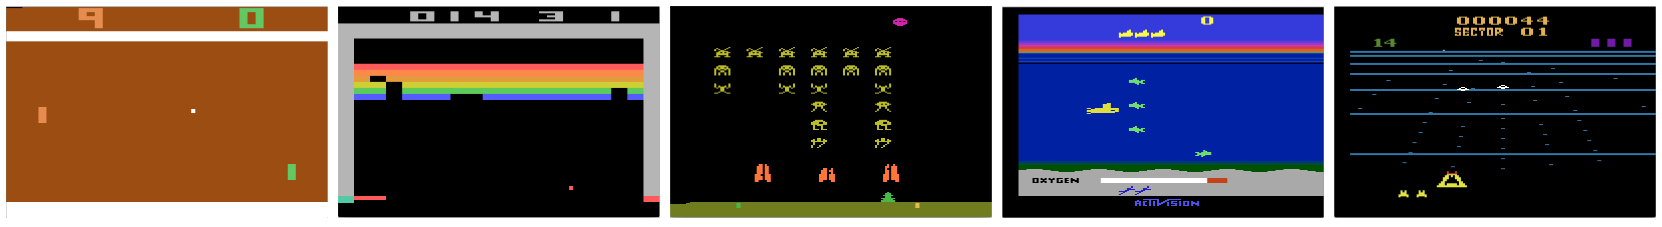
\includegraphics[width=\textwidth]{images/GRL.png}
    \caption{reinforcement learning Playing Atari Games \cite{mnih2013playing}.}
    \label{fig:GRL}
\end{figure}

\begin{figure}[h!]
    \centering
    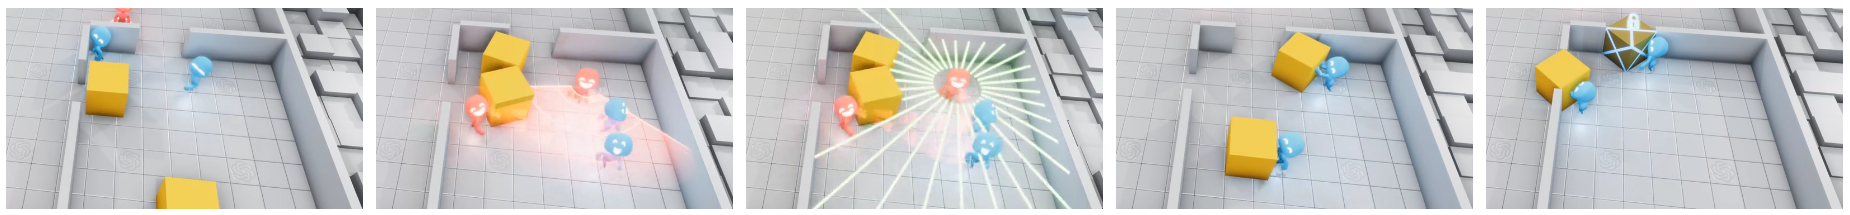
\includegraphics[width=\textwidth]{images/MARL.png}
    \caption{Cooperative Multi Agent reinforcement learning \cite{baker2020emergent}.}
    \label{fig:MARL}
\end{figure}

\begin{figure}[h!]
    \centering
    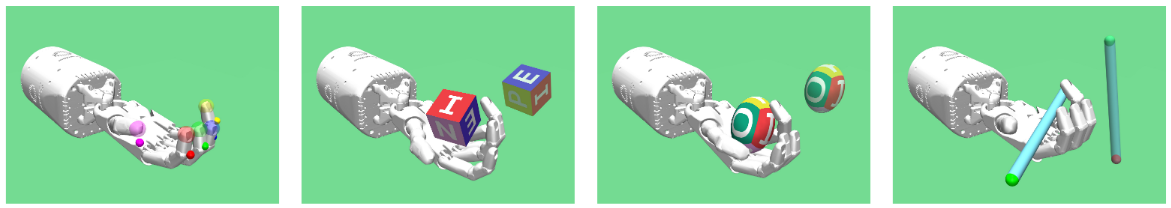
\includegraphics[width=\textwidth]{images/RRL1.png}
    \caption{Dexterous Robotic Manipulations by reinforcement learning in Simulation \cite{plappert2018multigoal}.}
    \label{fig:RRL1}
\end{figure}

\begin{figure}[h!]
    \centering
    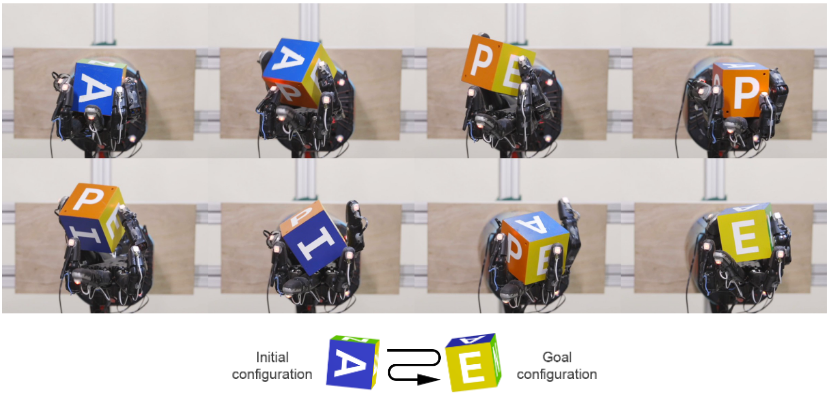
\includegraphics[width=\textwidth]{images/RRL.png}
    \caption{Dexterous Robotic Manipulations by reinforcement learning in Real World \cite{openai2019learning}.}
    \label{fig:RRL}
\end{figure}

So what makes it a challenge to apply reinforcement learning successfully to robotics? One of the main reasons is the nature of the environment itself. Unlike most games where the reward function can be directly optimized to reach the desired objective, robotics tasks are more indirect and goal-based. Most environments in the field of robotics, involve a component like an arm that interacts with an object in the environment to perform tasks like pushing, sliding, picking and placing etc. Given this scenario a direct reward function alone is not enough to train a policy as the task becomes more goal-oriented, naturally resulting in a case of sparse rewards as seen frequently in newly developed robotics environments. Binary and sparse rewards can be easily defined, for example, positive or zero rewards for completing a task and negative rewards for not completing a task. For robotics-based tasks, this kind of setup is more appropriate than a traditional reward function. Sparse rewards are also easier to work with for a reinforcement learning agent as it does not get stuck in a local minima, which is one of the problems that a well defined dense reward function faces. However, sparse rewards have their own set of unique challenges. The main problem of a sparse reward system compared to a dense reward system is that dense reward provides valuable information for every state the agent visits whereas sparse rewards provide meaningful information only when the agent completes a specific task. Without sufficient information from the reward, a randomly initialized agent with random exploration rarely sees any positive reward signal. The agent becomes sample inefficient and takes exceedingly many interactions with the environment to even see any positive feedback making it slow to converge and taking too long to learn. In some cases, the agent just fails to learn any meaningful actions, in other cases, the agent might end up learning undesirable behaviors which may be acceptable for a simulated environment but may not be suitable for real-world applications. Apart from the concerns of safety and failures, pure offline reinforcement learning also costs considerable time and hardware resources to train a successful policy. \\

Recent related research \cite{plappert2018multigoal} have been able to successfully implement complex tasks in robotics using reinforcement learning and sparse rewards. Using different exploration strategies like multi-agent and noise base exploration \cite{lanier2019curiositydriven}. Taking advantage of the off-policy nature of reinforcement learning algorithms and the experience replay memory trick to overcome these sparse rewards \cite{andrychowicz2018hindsight}. Also, using simulation-based tricks like initializing the environment in a much suitable situation for the agent. In this case, the agent can see a positive reward sooner helping in learning. These and other related researches have found success in reinforcement learning with sparse rewards. But, come with a cost either in the form of complex and difficult implementations, training time, and hardware resources. \\

The key takeaway from this is the need to reduce the training time and accelerate reinforcement learning in environments with complex dynamics like robotics, with a simple and straightforward implementation, without the need for heavy hardware resources or distributed computing. This is the main motivation behind this research. To achieve this the main area that needs to be addressed is the exploration phase of reinforcement learning which takes a major chunk of the training time. This time increases with the increase in complexity of the environment. \\

One of the approaches to overcome this limitation is to go for a supervised learning approach by using demonstrations sourced from an expert \cite{ARGALL2009469} \cite{RLFD} either in the form of imitation learning \cite{reddy2019sqil}  \cite{ILRL} or transfer learning \cite{Taylor2009TransferLF} \cite{TLMARLS} \cite{zhu2021transfer} \cite{ILTLRL}. Learning from Demonstrations or behavior cloning is a subset of imitation learning where demonstrations in the form of (state, action) tuple pair from an expert demonstrator are used as a form of supervised learning to induce the desired behavior and overcome random exploration resulting in higher performance than a randomly initialized agent. behavior cloning learns the mapping of the state-action pairs in the demo dataset and tries to mimic similar behavior to solve similar tasks. But, plain behavior cloning is restricted by the source, quality and quantity of the demonstrations. behavior cloning has shown great success \cite{BCAD} \cite{sumanth2020enhanced}, figure \ref{fig:BCAD} shows the application of behavior cloning for a self-driving car. However, in more complex environments behavior cloning is sometimes known to fail and result in undesirable behaviors. The reason for this is the limited number of demonstrations. behavior cloning takes advantage of demonstrations to solve tasks, but these demonstrations cannot be provided for each and every scenario, and this becomes increasingly difficult as the complexity of the task and environment increases. Also, behavior cloning suffers from a problem called the distributional drift problem, which is the difference in the distribution of the states of the learned policy and the distribution of the states of the expert policy in the demonstrations dataset causing errors that propagate over time resulting in catastrophic failures \cite{goecks2020integrating} \cite{codevilla2019exploring}. One way to solve these problems would be to combine behavior cloning with reinforcement learning, which in a sense complement each other by overcoming the other's limitations resulting in a more capable, safer and desirable policy acceptable in simulation and also suitable for real-world applications \cite{gao2019reinforcement} \cite{nair2018overcoming} \cite{vecerik2018leveraging}. Figure \ref{fig:BCRL} shows the combination of behavior cloning and reinforcement learning of a drone landing the Microsoft AirSim environment \cite{shah2017airsim}. \\

\begin{figure}[h!]
    \centering
    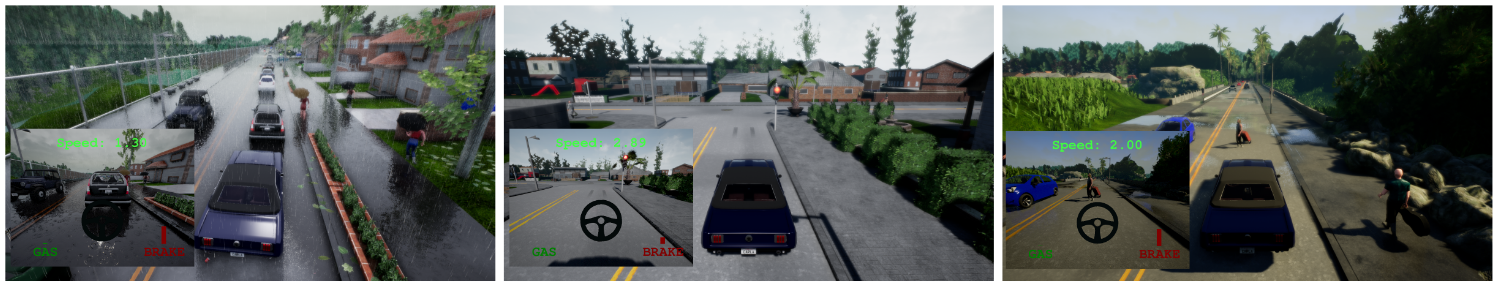
\includegraphics[width=\textwidth]{images/BCAD.png}
    \caption{behavior cloning used for Autonomous Driving \cite{codevilla2019exploring}.}
    \label{fig:BCAD}
\end{figure}

\begin{figure}[h!]
    \centering
    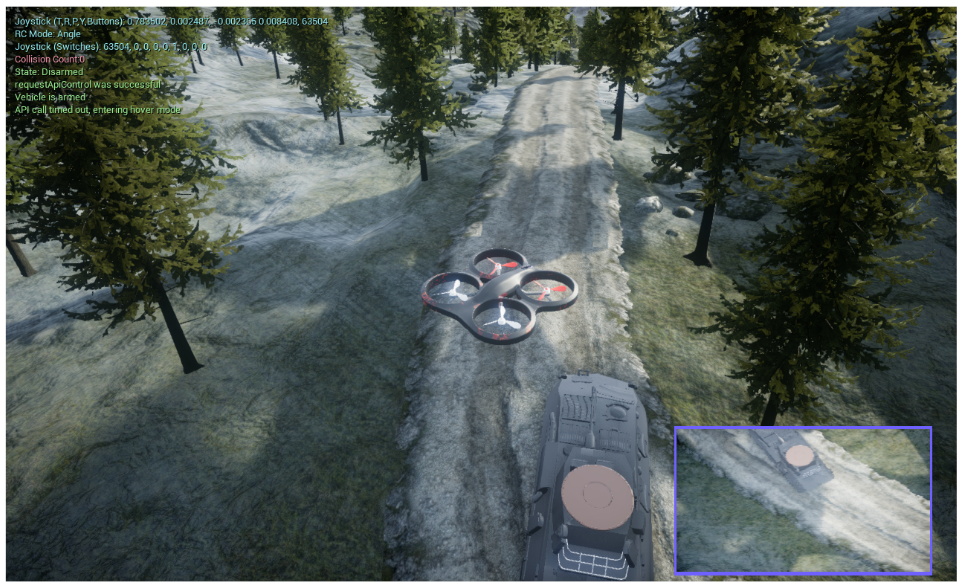
\includegraphics[width=\textwidth]{images/BCRL.png}
    \caption{behavior cloning and reinforcement learning used for Drone Landing \cite{goecks2020integrating}.}
    \label{fig:BCRL}
\end{figure}

Another approach in accelerating reinforcement learning and overcoming exploration is the reward function. Environments with sparse rewards do not provide enough information for the agent to explore properly and learn successfully. A randomly initialized agent with random exploration takes very long to get positive feedback increasing the training time overall. An over-engineered or well-defined reward function can result in sub-optimal policies hence the need for a well-crafted reward function. Previous research \cite{nagpal2020reward} \cite{Dewey2014ReinforcementLA} \cite{Konidaris2006AutonomousSK} have shown success in this area for complex environments and was enough motivation to pursue that direction as well in this research to develop a simple yet informative reward function in addition to the combination of behavior cloning and reinforcement learning methods mentioned above. \\

The contributions of this research paper are threefold. Firstly, this paper investigates the combination of behavior cloning and reinforcement learning with the most recent advances in the respective fields, by proposing a new loss function to combine the behavior cloning Imitation Learning Loss \cite{goecks2020integrating} \cite{nair2018overcoming} with the Actor-Critic based loss function \cite{lillicrap2019continuous} \cite{fujimoto2018addressing} of the reinforcement learning agent to accelerate the training. Secondly, this paper proposes a simple yet informative reward function to further aid the reinforcement learning agent in training. Thirdly, a training strategy to efficiently train the reinforcement learning agent using both the agent's data collected during exploration and the expert's data already collected as a part of the demonstrations dataset. By effectively using demonstrations from an expert as a part of the training process for a reinforcement learning agent, the learning can be accelerated even in complex environments. This proposed method has shown success compared to previous baselines and outperformed them. The agent is pretty robust to the source, quality and quantity of the demonstrations. The agent is not constrained or limited to the demo actions present in the dataset. The agent can develop new behaviors and can also outperform the expert demonstrator. The experiments are conducted and tested on the Open-AI Gym \cite{brockman2016openai} and MuJoCo \cite{MJC} based Fetch Robotics Environments \cite{plappert2018multigoal}. \\

\subsection{Research Questions}

The motivation behind this thesis has been explained in the previous section, the research will be focused on those areas and will be aiming to explore and answer the following themes. \\

\begin{itemize}[leftmargin=0.85in]
    \item[Q1.  ] \textbf{Can the proposed method successfully solve complex robotics tasks?} This is this first and foremost and most important question preceding the others, given the complex nature of the goal-based task and the dynamics of robotics environments, it would be essential to see if the proposed method can solve all the test environments successfully. \\

    \item[Q2.  ] \textbf{Does the proposed method achieve accelerated learning without a compromise to generalization?} This next question goes deep into the heart of this research. The main aim of this paper is the acceleration of reinforcement learning, hence this question has to be answered in two parts. The first would be to see if that acceleration is indeed achieved by the proposed method. Second, does this acceleration come at a cost, for example in the form of undesirable behaviors, or loss in generalization? \\

    \item[Q3.  ] \textbf{How does the proposed method compare to previous related baselines?} The final question is to gauge the performance of the proposed method by comparing this to previous related research, in terms of convergence rate and training time \textit{vs} hardware resources. \\
\end{itemize}

\subsection{Thesis Outline}

\textbf{Chapter 1} presents the introduction section where the reader is eased into the main theme of the research in this paper. Related concepts are introduced and the main motivation behind this research is presented. \\

\textbf{Chapter 2} goes into detail about the theoretical framework involved in structuring this research. Concepts will be explained in more detail and related research will be explored that have directly or indirectly influenced this research. \\

\textbf{Chapter 3} will look at the proposed methodology in detail, the architecture and algorithm involved in the current research will be explained along with the pseudocode for the framework. Simulators, toolboxes and environments used will be looked at in detail along with experiments conducted and hyperparameters used. \\

\textbf{Chapter 4} examines the results obtained from the experiments and comparisons will take place depending on the various performance criteria all of which will be explained in detail, followed by a discussion that will further explain what was observed and why with appropriate reasoning. \\

\textbf{Chapter 5} will finish this paper by summarizing the important concepts and focusing on the main contributions of this research, showcasing what was achieved, what went right, what went wrong and what could be done as an extension for future research. \\
